\documentclass[10pt]{article}
\usepackage[margin=0.60in]{geometry}
\usepackage{amsmath,booktabs,enumitem,fancyhdr,graphicx,listings,tabularx,titlesec,xcolor}
\usepackage[hidelinks]{hyperref}
\graphicspath{{docs/lessons/assets/}{../assets/}}
\hypersetup{
 pdftitle={ADK Lesson 063: An Inert Museum-Case Monitor},
 pdfauthor={Kevin Shanahan},
 pdfsubject={Composing copied liquid, thermal, radiant, reed, acknowledgement, and audit evidence into inert monitor intent},
 pdflang={en-US}}
\pagestyle{fancy}\fancyhf{}
\lhead{\textsc{ADK Lesson 063}}\rhead{Inert Museum-Case Monitor}
\cfoot{\thepage}\setlength{\headheight}{14pt}
\setlength{\parindent}{0pt}\setlength{\parskip}{3pt}
\setlist{nosep,leftmargin=1.45em}
\titleformat{\section}{\Large\bfseries}{\thesection}{0.5em}{}
\newcommand{\lessonbox}[1]{\begin{center}\fbox{\parbox{0.92\linewidth}{#1}}\end{center}}
\newcommand{\blankline}{\rule{0.76in}{0.4pt}}
\newcommand{\longblank}{\rule{1.35in}{0.4pt}}
\lstset{
 basicstyle=\ttfamily\footnotesize,
 columns=fullflexible,
 breaklines=true,
 frame=single,
 rulecolor=\color{black},
 showstringspaces=false}

\begin{document}
\small
\begin{center}
 {\Huge\bfseries An Inert Museum-Case Monitor}\\[3pt]
 {\Large Compose hazards without pretending to control hardware}\\[7pt]
 \fbox{\textbf{E0 SYNTHETIC REPLAY --- NO SENSOR, RELAY, OR STORAGE HARDWARE}}
\end{center}
\begin{tabularx}{\linewidth}{@{}>{\bfseries}l X >{\bfseries}l X@{}}
Lesson & 063 --- integrating project & Time & 180--240 minutes\\
Prerequisites & Lessons 061--062 and magnetic observations & Board & compile-only Mega replay\\
Input & one complete copied hazard frame & Observation & named intent and audit cells\\
\end{tabularx}

\lessonbox{\textbf{Responsibility.}
\texttt{MuseumCaseMonitor} composes copied liquid, thermal, radiant,
reed-contact, acknowledgement, and recorder evidence. It owns a deterministic
alarm/cooldown state machine, inert presentation and relay-lamp intent, and
one bounded audit transaction. It does not sample a sensor, switch a relay,
write storage, read an RTC, control access, or certify preservation or
safety.}

\section{Draw the boundary around policy}
The monitor begins with already-qualified copied observations. Lesson 061
provides liquid quality; Lesson 062 provides independent thermal and radiant
quality; a copied magnetic observation preserves the complete reed-contact
record. The operator acknowledgement and recorder receipt are copied evidence
too. Supplied time is the only clock.

\begin{center}
% ADK visual: pencil
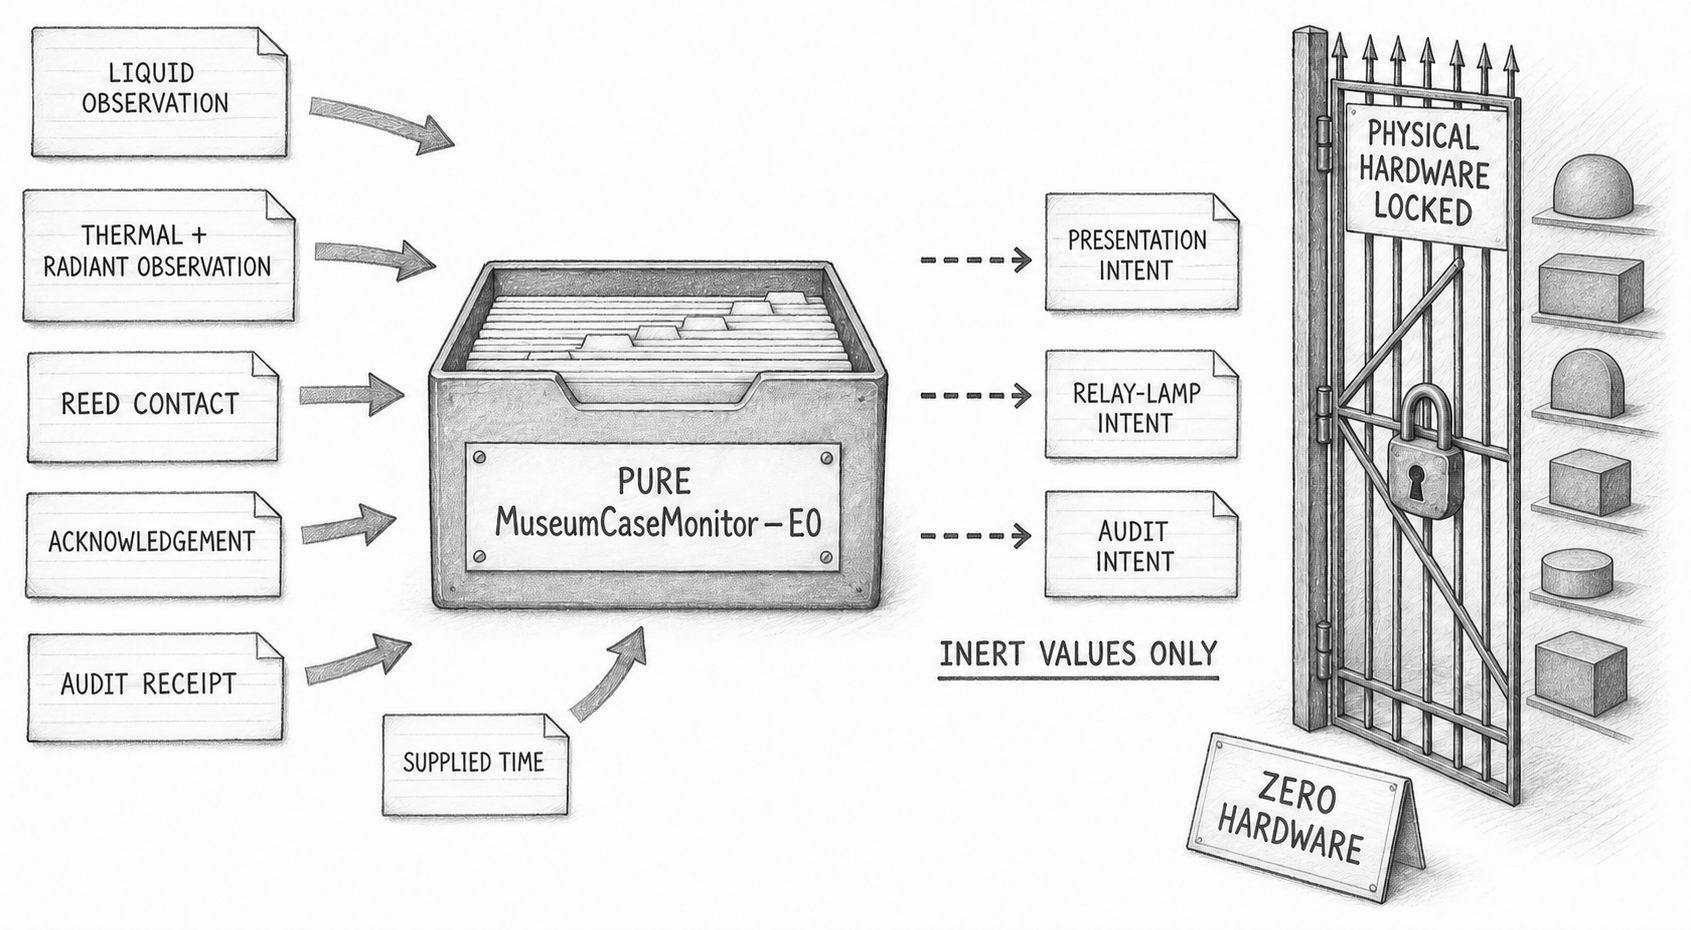
\includegraphics[width=0.96\linewidth,height=2.10in,keepaspectratio]
 {063-composition-boundary-pencil.png}

\small\textit{Alternative text: a pencil drawing feeds six copied evidence
cards into an inert museum-case policy; a locked physical gate separates the
policy from unidentified sensors, display, sounder, relay lamp, RTC, and
storage, and no wire crosses the gate.}
\end{center}

\begin{tabularx}{\linewidth}{@{}X X@{}}
\toprule
E0 proves & E0 does not prove\\
\midrule
hazard precedence and cooldown from copied evidence & simultaneous physical sampling\\
inert RGB, LCD, sound, and relay-lamp intent & any energized output or safe electrical state\\
one bounded recorder intent/receipt transaction & durable storage or wall-clock accuracy\\
deterministic replay and attribution & fire detection, security, or preservation fitness\\
\bottomrule
\end{tabularx}

There is no formal electrical schematic at E0. An authoritative schematic
requires every exact specimen, independent electrical qualification, resource
and safe-state evidence, and measured combined acceptance. A generic relay or
sensor drawing would conceal the open work rather than teach it.

\section{Keep the complete hazard frame attributable}
Every frame names the exact expected source and revisions fixed by
\texttt{MuseumCaseConfig}. The liquid and environment values preserve their
complete Lesson 061 and 062 observations. The reed wrapper preserves the
complete qualified magnetic observation, not merely a Boolean. A qualified
active contact means case closed; qualified inactive means reed-open and
case-open, producing the \texttt{Opening} hazard.

\begin{center}
% ADK visual: pencil
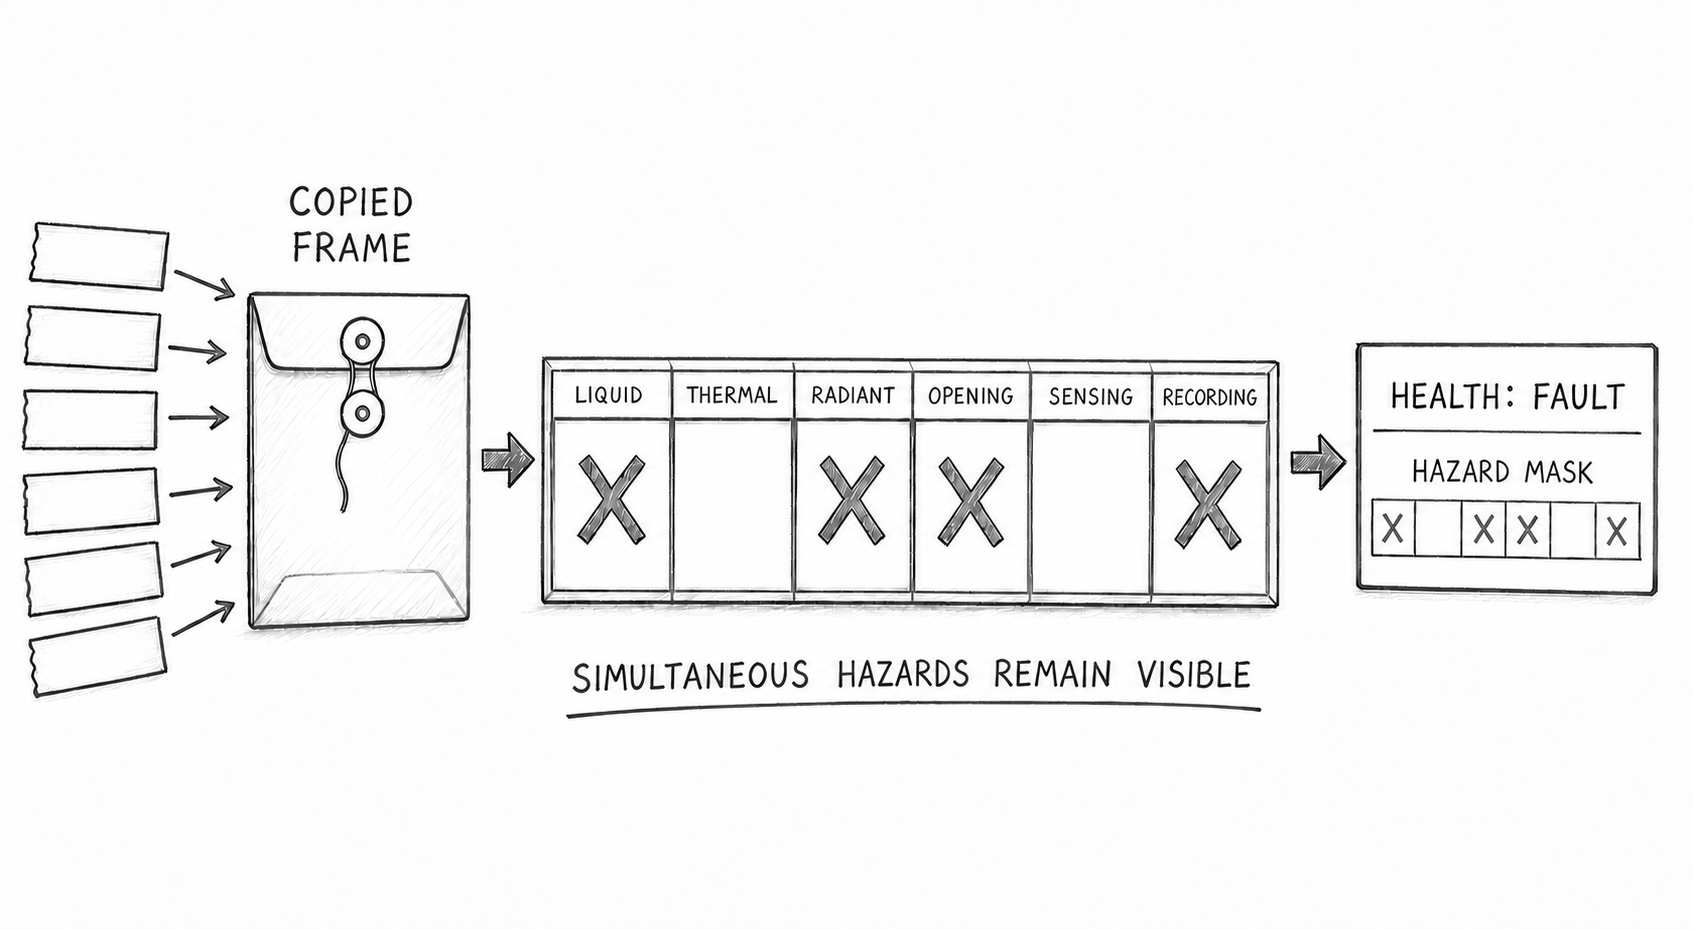
\includegraphics[width=0.96\linewidth,height=2.20in,keepaspectratio]
 {063-hazard-frame-pencil.png}

\small\textit{Alternative text: a hand-drawn additive hazard ledger retains
liquid, radiant, opening, and recording bits together; recording makes the
reported health fault without erasing the other hazard evidence.}
\end{center}

Structural validation precedes interpretation. Zero or duplicate role IDs,
wrong revisions, unknown enum/status encodings, future or modularly ambiguous
times, ordering violations, and mismatched receipt fields reject atomically.
A convincingly alarming value cannot rescue an invalid frame. By contrast, a
structurally valid but too-old required observation is admitted as evidence of
a sensing problem: it commits \texttt{Fault} with the \texttt{Sensing} bit.
Ordinary unsigned rollover with a wrap-valid age follows that same semantic
age rule rather than being rejected merely because the counter wrapped.

\begin{tabularx}{\linewidth}{@{}l X@{}}
\toprule
Evidence & Why the monitor retains it\\
\midrule
six producer sequences & audit witness attribution and replay\\
independent observation times and ages & delayed sources are not called simultaneous\\
reed polarity, raw level, quality, and edges & case-open meaning is not reduced to a bare bit\\
operator source, sequence, time, and status & acknowledgement remains attributable intent\\
\bottomrule
\end{tabularx}

Predict the result when the reed Boolean appears closed but its copied
magnetic quality is faulted: health \blankline; sensing hazard present?
\blankline.

\section{Apply fault and hazard precedence}
For a valid frame, lifecycle state first prevents active output intent. A
sensing fault or stale required source produces \texttt{Fault}, never
\texttt{Healthy}. Wet liquid, thermal alarm, radiant hazard, or case-open
evidence latches \texttt{Alarm}. Lesser damp, uncertainty, or disagreement
conditions produce \texttt{Warning}.

\begin{center}
% ADK visual: pencil
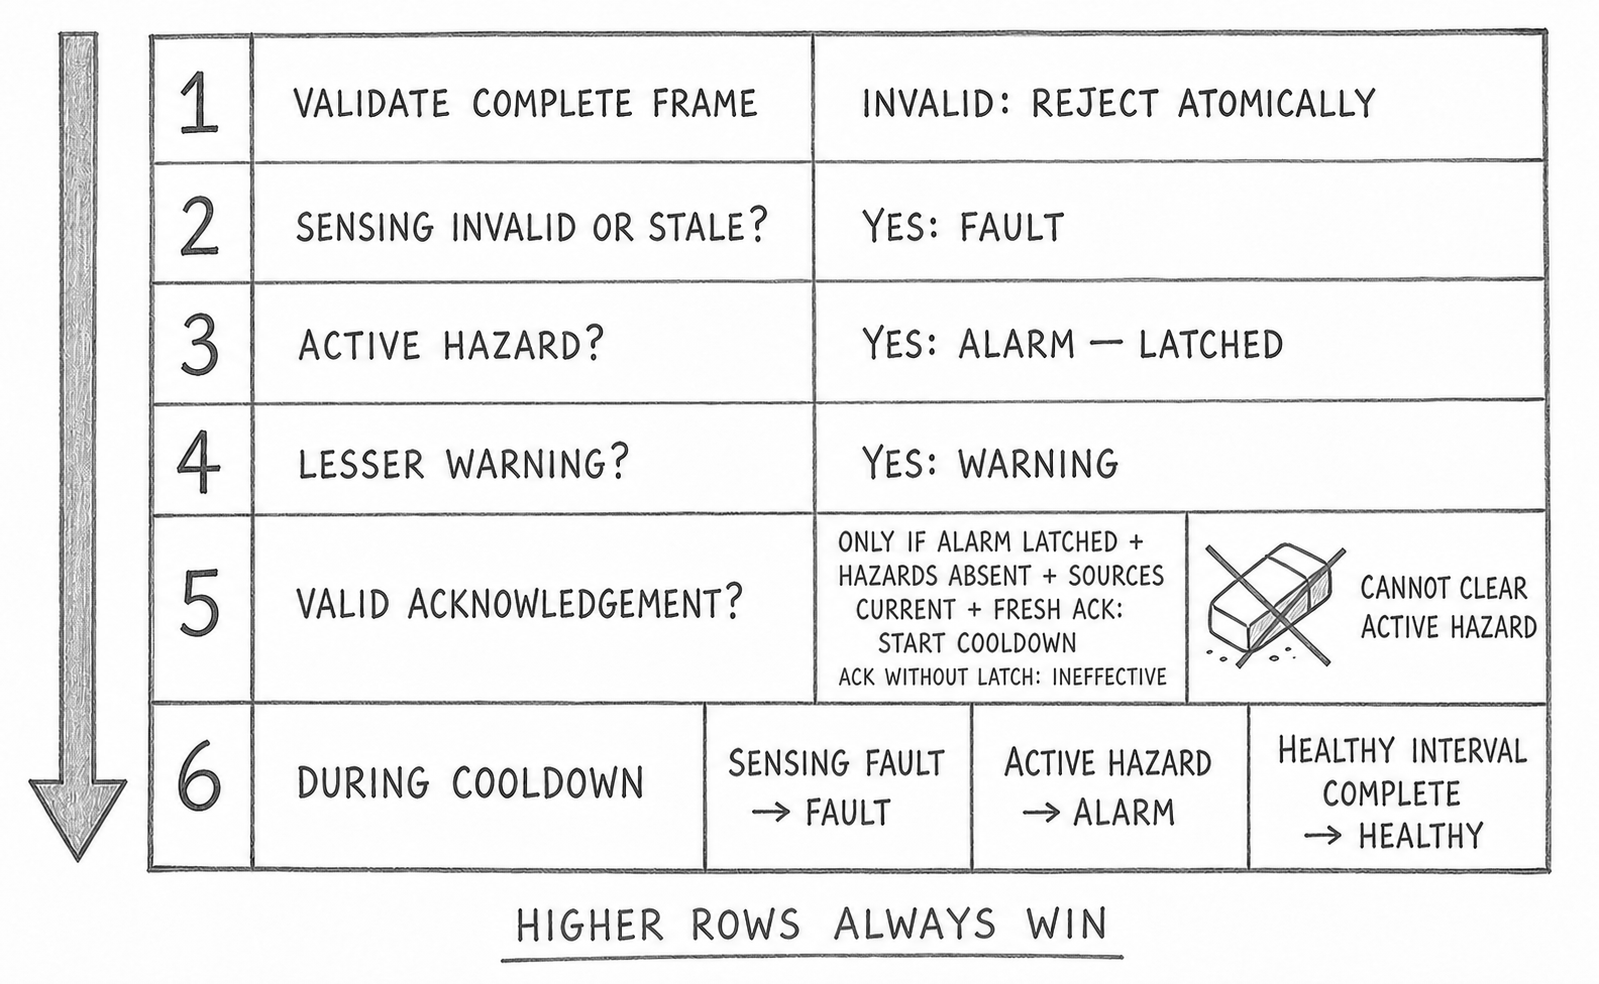
\includegraphics[width=0.95\linewidth,height=2.25in,keepaspectratio]
 {063-precedence-ladder-pencil.png}

\small\textit{Alternative text: a pencil precedence ladder checks frame
validation, sensing faults, active hazards, lesser warnings, the latched-alarm
and fresh-acknowledgement condition, and cooldown interruption or completion.}
\end{center}

\begin{tabularx}{\linewidth}{@{}l l X@{}}
\toprule
Condition & Health & Hazard evidence retained\\
\midrule
stale or invalid required sensing & \texttt{Fault} & \texttt{Sensing} plus other supported bits\\
wet, thermal alarm, radiant hazard, or open case & \texttt{Alarm} & every simultaneous hazard bit\\
damp, thermal warning, or disagreement & \texttt{Warning} & lesser condition remains attributable\\
first complete clean frame, with no prior alarm latch & \texttt{Healthy} & none\\
clean recovery from a latched alarm after acknowledgement & \texttt{Cooldown} & none\\
clean latched-alarm recovery after cooldown & \texttt{Healthy} & none\\
\bottomrule
\end{tabularx}

A single highest-alarm enum would lose collisions. The hazard mask therefore
retains \texttt{Liquid}, \texttt{Thermal}, \texttt{Radiant},
\texttt{Opening}, \texttt{Sensing}, and \texttt{Recording} independently.
If liquid and opening alarms arrive together, record the expected health
\blankline\ and hazard combination \longblank.

\section{Acknowledge only after hazards clear}
Acknowledgement records operator intent; it cannot clear an active hazard or
sensing fault. Cooldown exists only to recover a previously latched alarm.
After that alarm's hazards are absent and every required source is current, a
fresh acknowledgement starts the configured cooldown. An acknowledgement
when no alarm is latched is ineffective and cannot move a first clean frame
away from \texttt{Healthy}. Any hazard or sensing fault during cooldown
relatches alarm or fault. A lesser warning interrupts cooldown and reports
\texttt{Warning}; a later clean frame still needs a fresh acknowledgement
before recovery can restart. Only a complete clean cooldown returns the
latched monitor to \texttt{Healthy}.

\begin{center}
% ADK visual: pencil
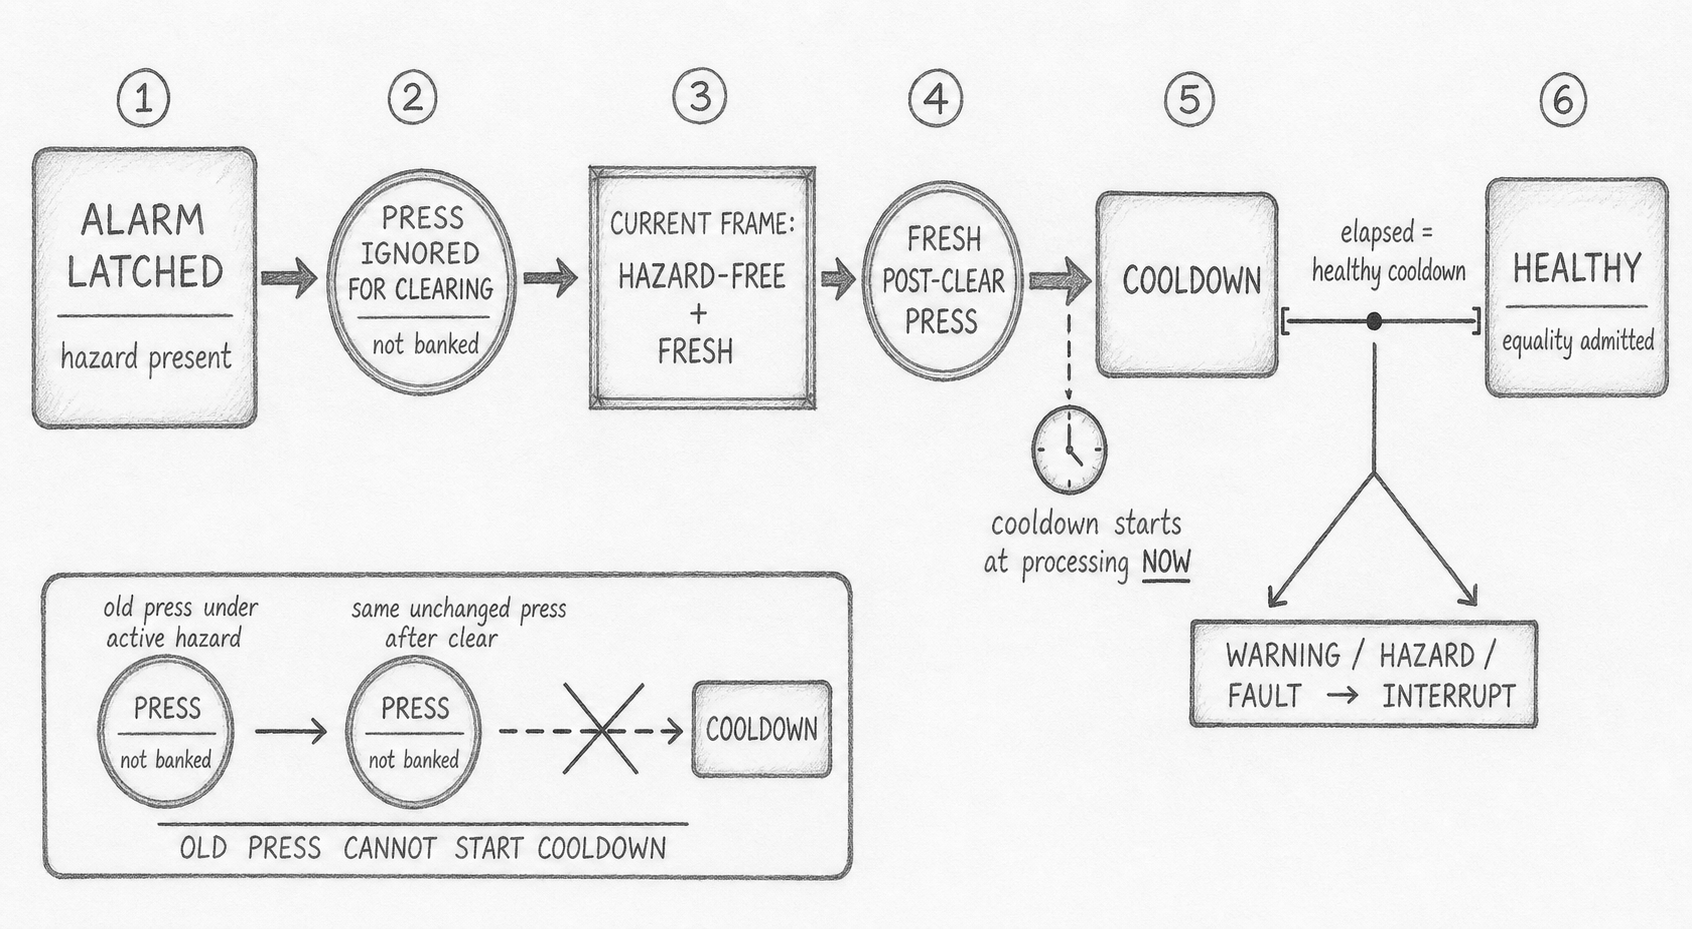
\includegraphics[width=0.95\linewidth,height=2.05in,keepaspectratio]
 {063-alarm-cooldown-pencil.png}

\small\textit{Alternative text: a pencil state trace moves from qualifying to
alarm, ignores acknowledgement while a hazard remains, enters cooldown only
after clean evidence and acknowledgement, interrupts on warning, relatches on
a new hazard, and reaches healthy only after a restarted complete clean
cooldown.}
\end{center}

\begin{enumerate}
 \item First complete clean frame with a pressed acknowledgement:
       \blankline.
 \item Alarm plus pressed acknowledgement: health remains \blankline.
 \item Clean current frame after that alarm plus a fresh press: next state
       \blankline.
 \item Warning one tick before cooldown completion: next state \blankline.
 \item Clean evidence exactly at the restarted cooldown boundary: admitted or delayed?
       \blankline.
 \item Repeated ineffective acknowledgement with unchanged semantics: creates
       a new audit decision? \blankline.
\end{enumerate}

\texttt{initialize(now)} advances the nonzero lifecycle generation and
publishes qualifying, inactive outputs. \texttt{reset(now)} advances it again,
invalidates old receipts, clears volatile retry/cooldown history, and returns
to qualifying without claiming present hazards were cleared.
\texttt{shutdown()} invalidates audit state and publishes canonical inactive
outputs; repeated shutdown is idempotent.

\section{Publish intent, not hardware effects}
The output is a \texttt{MuseumCaseIntent}: health, complete hazard mask,
grayscale-safe RGB blink code, LCD age-or-fault visibility, sound intent,
inert relay-lamp intent, and an explicit inactive-alarm-output flag.

\begin{center}
% ADK visual: pencil
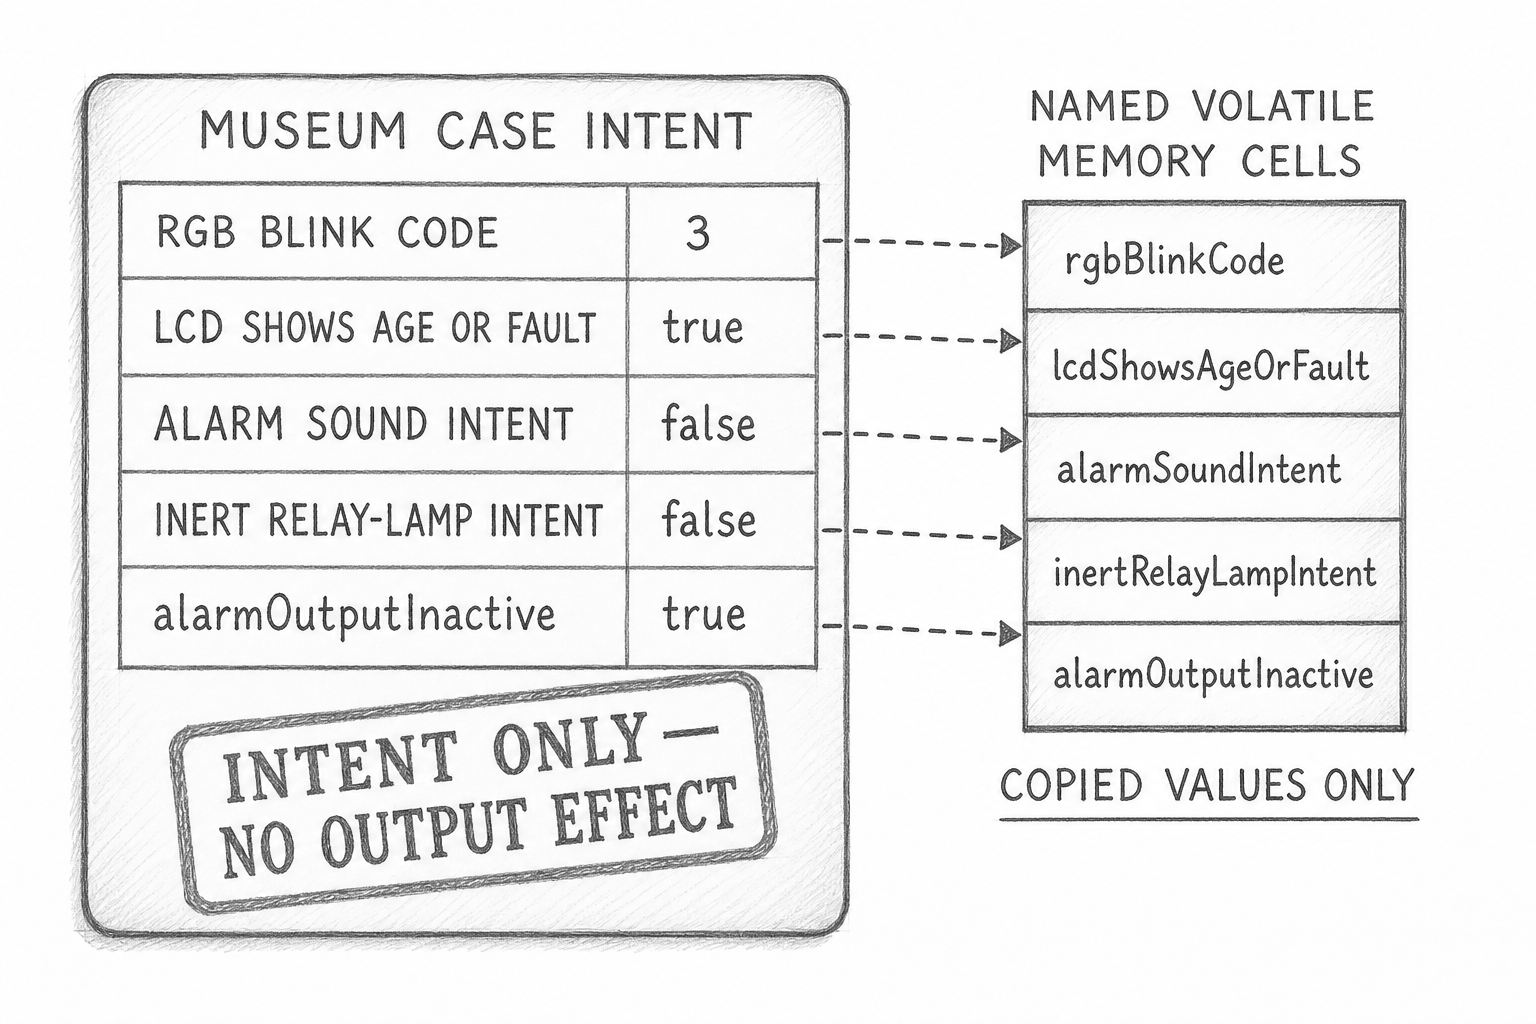
\includegraphics[width=0.95\linewidth,height=1.95in,keepaspectratio]
 {063-inert-output-intent-pencil.png}

\small\textit{Alternative text: a pencil intent card copies RGB blink code,
LCD age-or-fault visibility, alarm-sound intent, inert relay-lamp intent, and
alarm-output-inactive into matching named volatile memory cells under an
explicit no-output-effect stamp.}
\end{center}

Shutdown and every not-initialized result require sound and relay-lamp intent
false and \texttt{alarmOutputInactive} true. These values do not prove that a
physical output became inactive. Future E1c/E1d work must prove the
presentation endpoints and combined passive fixture; E2 may qualify only an
extra-low-voltage, current-limited inert lamp behind an independently
removable supply.

The relay may never control mains, a lock, access, confinement, egress, or a
safety load. RGB, LCD, and sound intent are diagnostic presentation, not
security or life-safety signaling.

\section{Freeze one audit witness at a time}
Every record-creating semantic decision publishes at most one outstanding
\texttt{MuseumAuditIntent}. Its immutable witness includes owner, lifecycle
and configuration, record sequence, observation time, health and hazard mask,
all six producer sequences, and a 32-bit FNV-1a digest. Delivery
\texttt{issuedAt} and attempt are not part of the event witness.

\begin{center}
% ADK visual: pencil
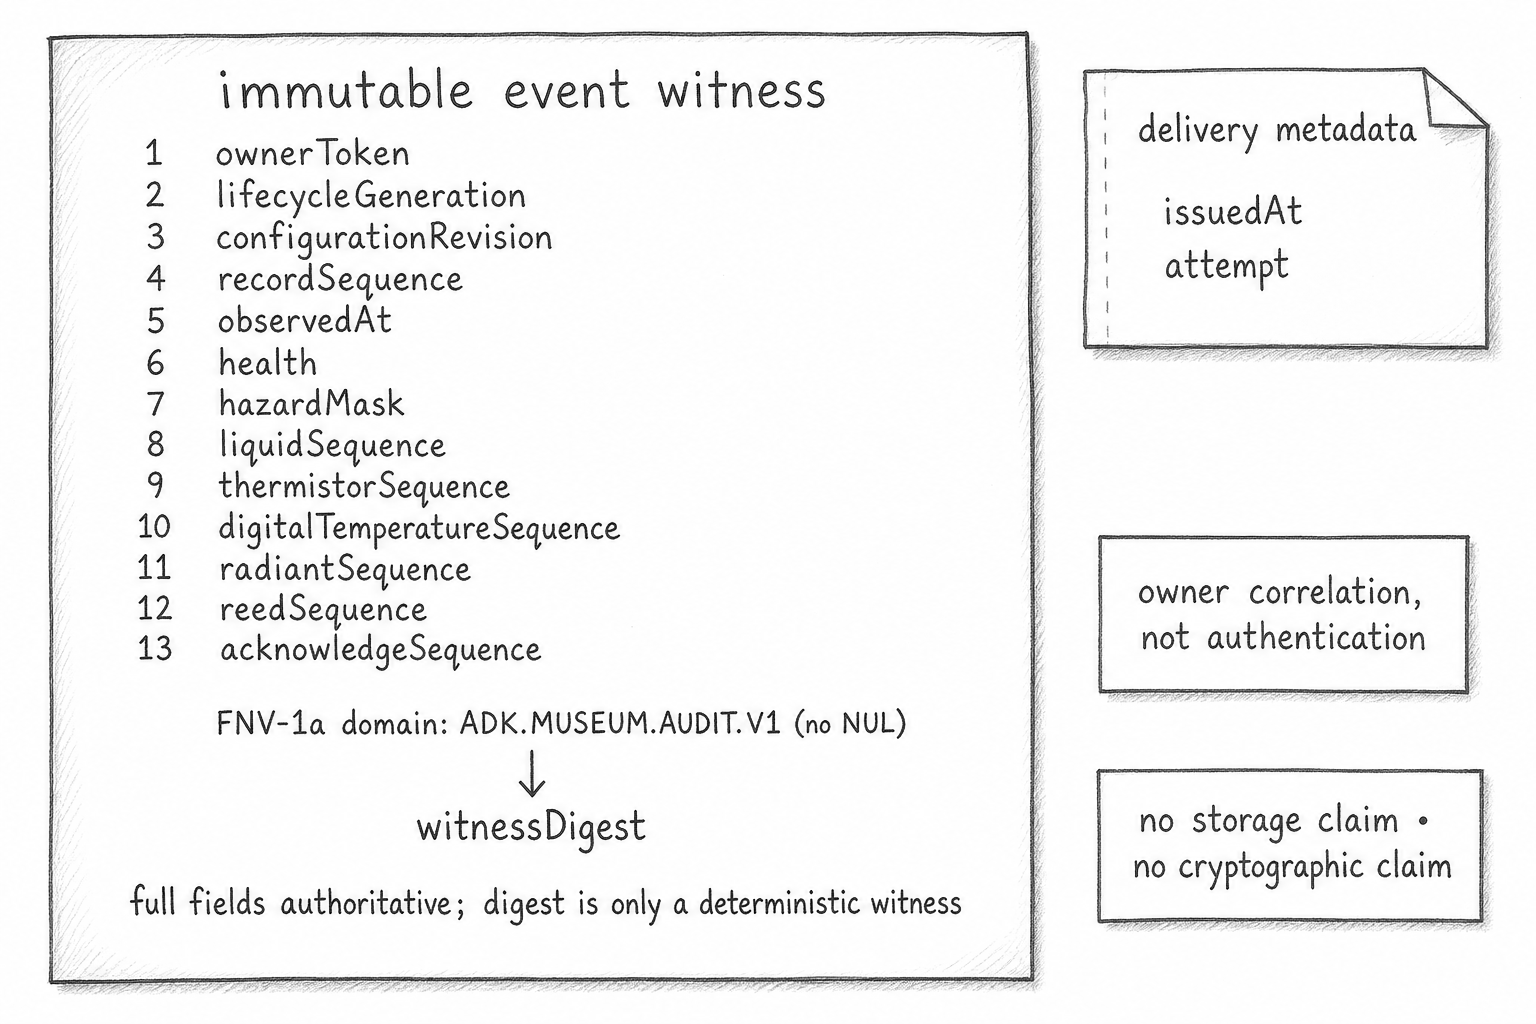
\includegraphics[width=0.96\linewidth,height=2.25in,keepaspectratio]
 {063-audit-witness-pencil.png}

\small\textit{Alternative text: a pencil audit card seals owner, lifecycle,
configuration, record, observation time, health, hazard mask, and six source
sequences beneath one witness digest, while issued-at and attempt sit on a
replaceable delivery tab outside the seal.}
\end{center}

The digest runs FNV-1a over ASCII \texttt{ADK.MUSEUM.AUDIT.V1} without its
terminating NUL, followed by the canonical fields in fixed order. Integers are
little-endian; enum and mask values use one byte. Full witness fields are
always compared, so the digest never substitutes for the record.

The frozen test vector uses owner \texttt{0x01020304}, lifecycle
\texttt{0x11223344}, configuration \texttt{0x5566}, record
\texttt{0x778899aa}, observed milliseconds \texttt{0x0a0b0c0d}, health
\texttt{Alarm}, hazard mask \texttt{0x19}, and producer sequences
\(\{1,2,3,4,5,6\}\). Predict the frozen digest before checking the test:
\texttt{0x}\longblank. The canonical answer is \texttt{4086e509}.

The first complete sensed decision after initialize or reset creates a
record. A clean first frame is \texttt{Healthy}; depending on its evidence,
the first decision may instead be \texttt{Warning}, \texttt{Alarm},
\texttt{Fault}, or evidence-driven \texttt{Qualifying}. Initial
\texttt{Cooldown} is unreachable because no alarm has yet been latched.
Later record creation uses the exact semantic key
\(\{\text{health},\text{hazard mask}\}\). A fresh same-key sample updates live
provenance but does not manufacture a record. Every health or hazard-mask
change does.

\section{Retain the latest successor during delivery}
The monitor has one outstanding immutable record and one
\texttt{dirtySuccessor} slot. If decisions change while delivery is pending,
the outstanding witness remains frozen and the slot retains the latest net
decision. Several changes may coalesce only to that latest bounded successor.
The slot obeys three complete rules on every valid frame:
\begin{enumerate}
 \item if the current semantic key returns to the outstanding record's key,
       clear the dirty slot because there is no net successor;
 \item if the key still matches the dirty slot, refresh the slot's complete
       current witness fields, including the latest producer sequences and
       observation time;
 \item otherwise replace the slot with the complete current decision.
\end{enumerate}
The slot has no record sequence, digest, attempt, or deadline until promotion.

\begin{center}
% ADK visual: pencil
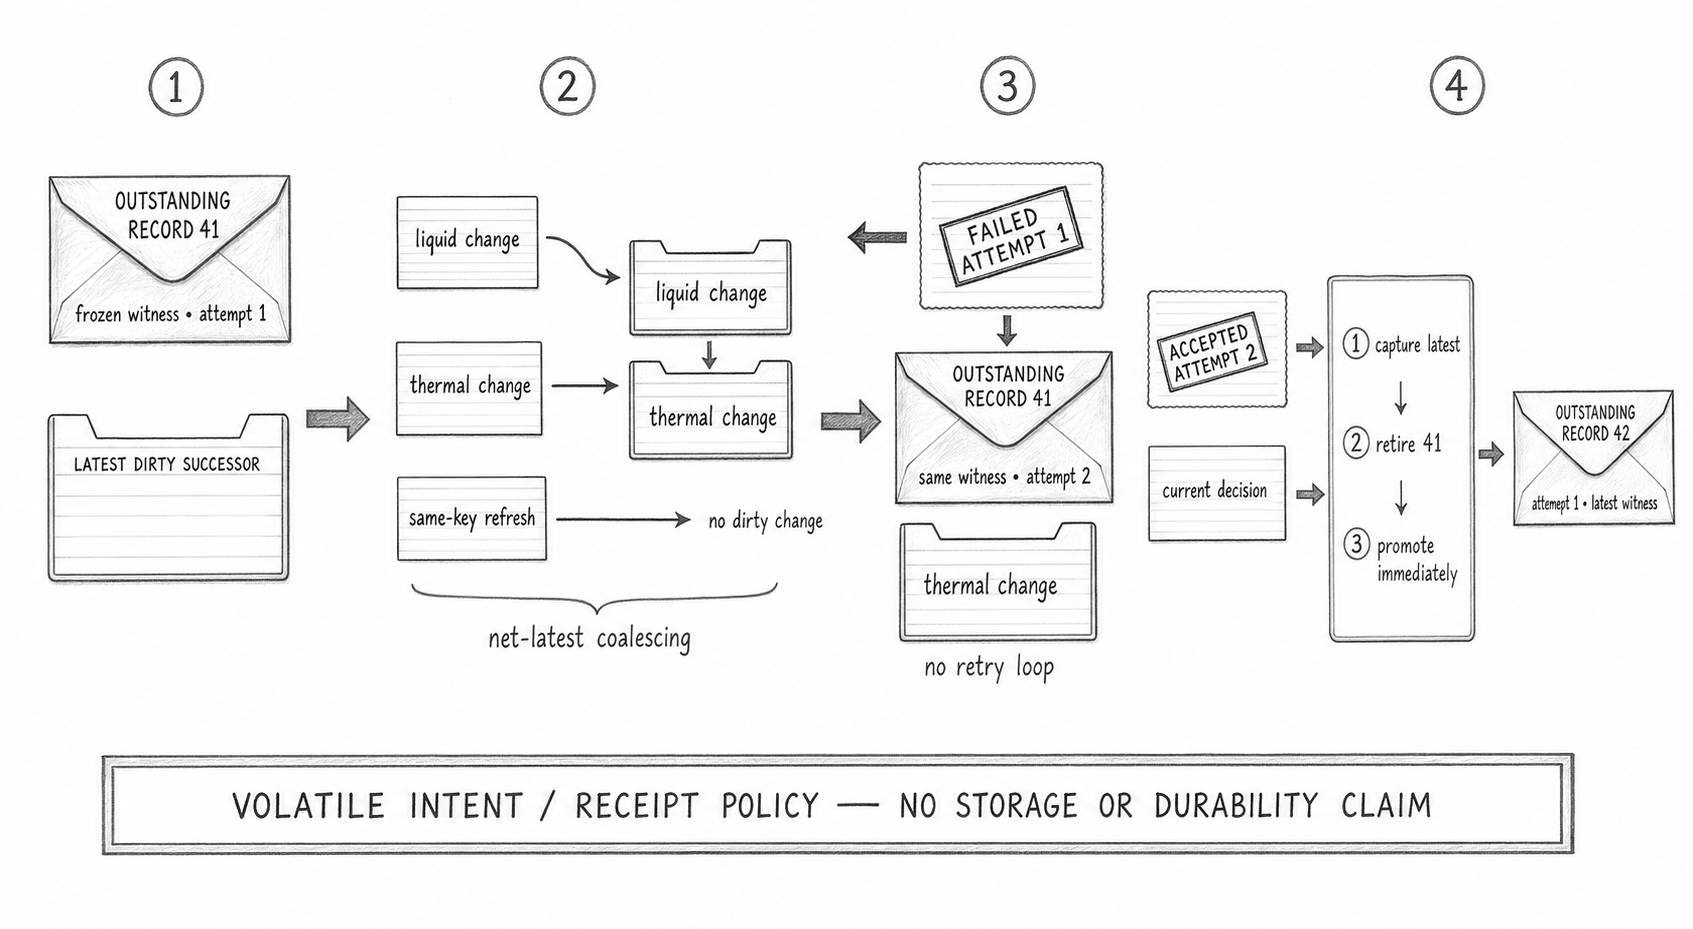
\includegraphics[width=0.96\linewidth,height=2.20in,keepaspectratio]
 {063-audit-collision-pencil.png}

\small\textit{Alternative text: a pencil sequence keeps audit record 41
sealed while liquid then thermal changes replace one latest dirty successor;
a failed first attempt retains both, and an accepted attempt-two receipt
retires 41 and immediately promotes the latest card as record 42.}
\end{center}

A receipt must match the owner, lifecycle, configuration, record sequence,
every witness field, digest, and current attempt. Acceptance retires the
record. Failure or deadline loss adds \texttt{Recording}, increments the
bounded attempt, and later reissues the same witness. There is no retry loop.
The inclusive deadline remains pending; the next valid tick records loss.

When an accepted receipt and a changed decision arrive together, validation
and latest-successor capture occur first. Then the receipt retires the old
record and the successor is immediately assigned the next sequence, digest,
deadline, and attempt one. This order prevents the newest decision from being
silently treated as covered by an older receipt.

\begin{tabularx}{\linewidth}{@{}l X@{}}
\toprule
Collision & Required result\\
\midrule
current key equals outstanding key & clear any dirty successor\\
current key equals dirty key & refresh its complete latest witness\\
current key differs from both & replace with complete current decision\\
several key changes while pending & one net-latest complete successor retained\\
failed receipt with successor present & immutable record and successor both retained\\
accepted receipt plus current change & retire old; immediately publish latest successor\\
final attempt fails & freeze both, assert recording fault, emit no retry\\
\bottomrule
\end{tabularx}

Only explicit reset or shutdown may discard terminal volatile audit state;
that discard is never reported as storage success. RTC accuracy, media
durability, atomic file commit, wear, and recovery after power loss remain
deferred physical work.

\section{Replay the complete collision trace}
The Mega sketch feeds copied result cells into one monitor. The caller owns
the result buffer passed to \texttt{update}; the monitor neither allocates nor
returns a hidden aggregate. The sketch does not call storage or acquire
hardware.

\begin{lstlisting}
MuseumCaseMonitor monitor (config);
monitor.initialize (TimePoint (0));

MuseumCaseResult result = {};
result.intent            = monitor.snapshot ();
const Status updateStatus = monitor.update (frame, result);
if (updateStatus.ok () && result.hasAuditIntent) {
    auditIntentResult = result.auditIntent;
}
if (updateStatus.ok ()) {
    intentResult = result.intent;
}
\end{lstlisting}

\begin{center}
% ADK visual: pencil
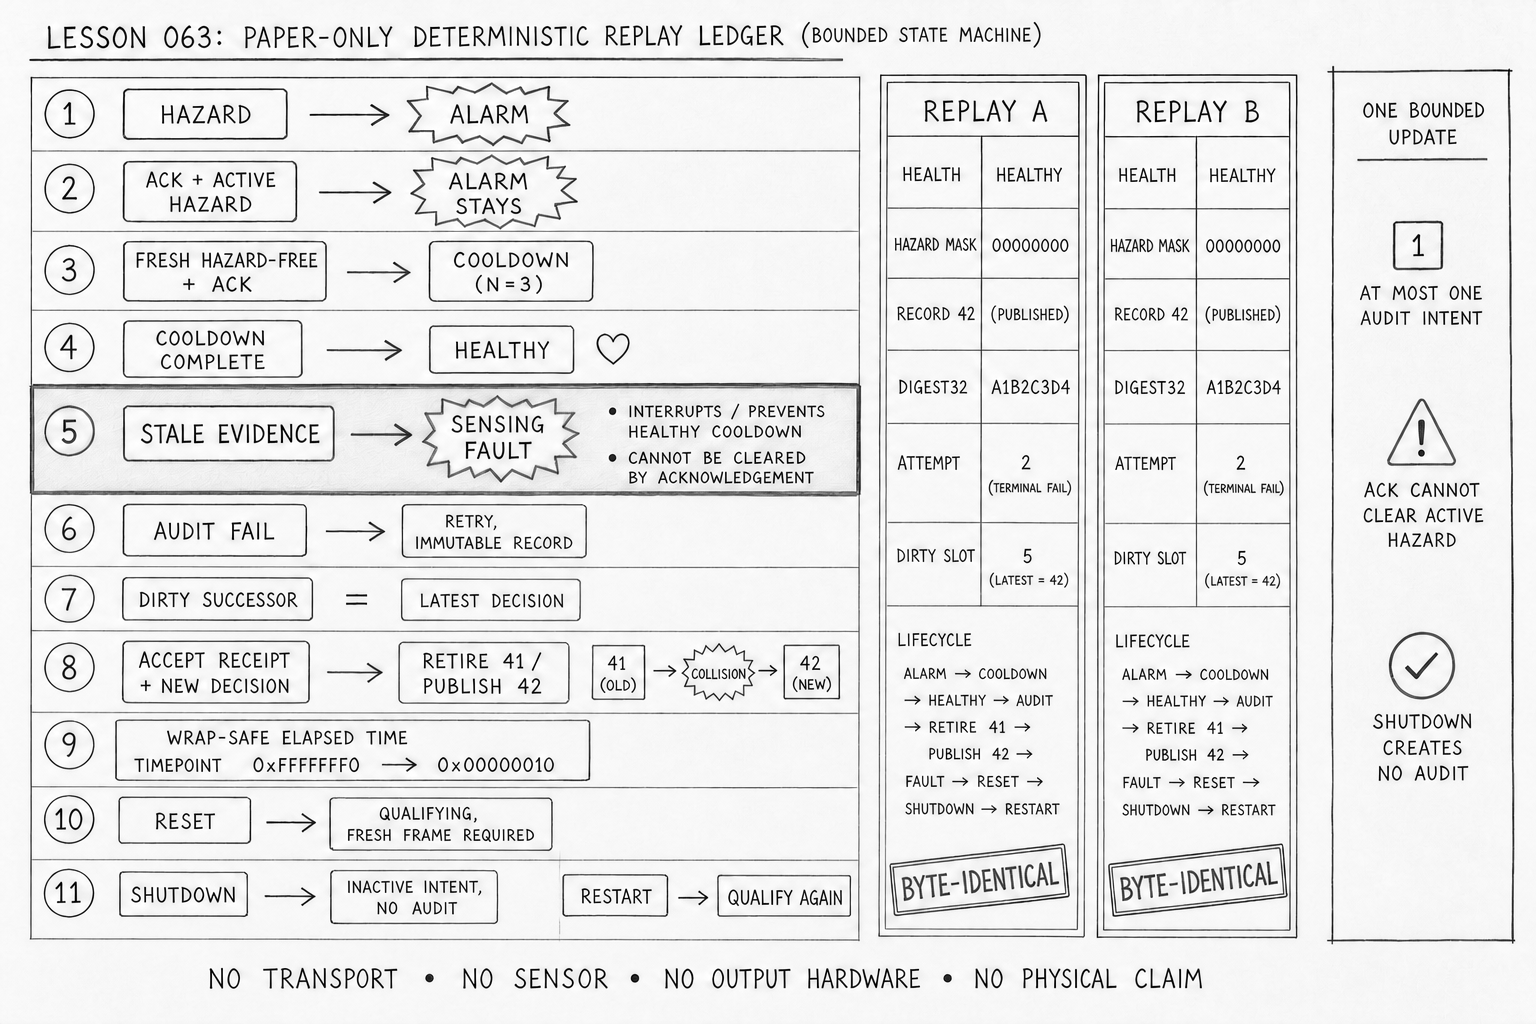
\includegraphics[width=\linewidth,keepaspectratio]
 {063-replay-ledger-pencil.png}

\small\textit{Alternative text: a pencil replay ledger covers first complete
decisions, simultaneous hazards, stale sensing, ineffective acknowledgement,
cooldown, record 41, failed delivery, changing successor, accepted receipt,
record 42, terminal retry exhaustion, reset, rollover, and shutdown in named
result cells.}
\end{center}

The canonical collision starts with alarm record 41, changes liquid and
thermal evidence during attempt one, fails that attempt, changes radiant and
case-opening evidence during attempt two, then accepts attempt two in the same
update as acknowledgement changes. Record 42 must contain the latest six
producer sequences and hazard state, not either intermediate witness.

Complete these diagnoses:
\begin{enumerate}
 \item Wrong digest but otherwise matching receipt: \longblank.
 \item Matching receipt one tick after inclusive deadline: \longblank.
 \item Accepted retired receipt repeated byte-for-byte: \longblank.
 \item Record sequence would wrap to zero: \longblank.
 \item Shutdown with an outstanding record: output becomes \longblank; storage
       success claimed? \blankline.
\end{enumerate}

\section{Inspect gates and record evidence}
\begin{tabularx}{\linewidth}{@{}l X X@{}}
\toprule
Gate & E0 evidence & Still open\\
\midrule
composition & exhaustive hazard and cooldown replay & simultaneous powered sensing\\
outputs & inert intent and inactive lifecycle results & endpoint acquisition and safe electrical state\\
audit & witness, collision, receipt, retry, and reset traces & durable media and wall-clock behavior\\
resources & exact compiler and object/stack gate & physical current and combined rail budget\\
observation & named volatile result cells & RGB/LCD/sound/relay physical evidence\\
\bottomrule
\end{tabularx}

The ordinary Mega replay measures 21,348 bytes of flash and 1,405 bytes of
static SRAM. The isolated no-LTO resource gate measures 22,980 bytes of flash,
1,405 bytes of static SRAM, and 819 bytes of conservative synchronous stack.
Aggregate policy objects occupy 709 bytes: 528 for the monitor, 69 for the
Lesson 061 policy, and 112 for the Lesson 062 policy. The caller-owned
envelope and result buffers occupy 207 and 72 bytes respectively; each passes
the 256-byte per-buffer limit, while their combined footprint is 279 bytes.
After the specified reserve and stack accounting, 5,840 bytes of Mega SRAM
remain.

The scoped evidence fingerprint is
\texttt{1c9a3bcbbf4883f9583ab2b5593cf1e507c5cc476200593d010b5c6ef371aaff}.
Every flash, SRAM, stack, object, caller-buffer, residual, ownership, and
hidden-return hard gate passes; the 819-byte stack result is an independently
reviewed target miss below the 896-byte hard limit. The ordinary
sketch and isolated no-LTO probe are separate measurement boundaries; their
flash and static-SRAM numbers must not be added.

\lessonbox{\textbf{Physical gates remain open.}
E1c qualifies the exact reed and harmless presentation endpoints. E1d proves
the combined passive monitor, including current, rail, source age,
disagreement, shutdown, and non-Serial observation. E2 may qualify only an
extra-low-voltage, current-limited inert relay/lamp fixture with independent
power removal. No mains, flame, heater, ignition, laser, lock, access,
confinement, egress, preservation, or life-safety function is authorized.}

\begin{tabularx}{\linewidth}{@{}X X@{}}
\toprule
Completion check & Result or evidence\\
\midrule
Exact identities, nested provenance, and atomic frame validation & \\
\addlinespace[1.1em]
Every health transition and hazard-mask add/remove combination & \\
\addlinespace[1.1em]
Acknowledgement, cooldown boundaries, relatch, reset, and shutdown & \\
\addlinespace[1.1em]
Frozen witness vector, digest, receipt matching, and deadlines & \\
\addlinespace[1.1em]
Dirty successor, collision order, retry exhaustion, and rollover & \\
\addlinespace[1.1em]
Canonical resource gate and reviewed target dispositions & \\
\addlinespace[1.1em]
Zero-hardware E0 boundary and all E1c/E1d/E2 gates & \\
\addlinespace[1.1em]
\bottomrule
\end{tabularx}

\begin{center}
\fbox{\parbox{0.90\linewidth}{
\textbf{Completion statement:} I can preserve simultaneous and attributable
hazards, explain why acknowledgement cannot clear active evidence, replay the
bounded audit transaction and collision order, and identify every physical
claim that remains open.

\vspace{0.10in}
Learner: \longblank\quad Reviewer: \longblank\quad Date: \blankline
}}
\end{center}

This print edition is untagged. Its text is searchable and copyable, and the
HTML lesson provides the hardware-independent alternative. No PDF/UA, WCAG,
or other PDF accessibility-conformance claim is made.

\end{document}
